%%% Esqueleto base de la presentacion
%%% No agregar las paginas con un include
%%% Lo que quieran aportar deben ser usuarios del TRAC

\documentclass{beamer}
\usepackage[spanish,activeacute]{babel}
\usepackage[utf8]{inputenc}
\usepackage{listings}
\usepackage{color}
\usepackage{tikz}
\usepackage{pgf}

\definecolor{red}{RGB}{255,0,0}
\definecolor{green}{RGB}{0,255,0}
\definecolor{blue}{RGB}{0,0,255}
\definecolor{oran}{RGB}{255,93,0}

\newcommand{\blue}{\textcolor{blue}}
\newcommand{\red}{\textcolor{red}}
\newcommand{\green}{\textcolor{green}}
\newcommand{\oran}{\textcolor{oran}}
\newcommand{\gray}{\textcolor{gray}}

\usetheme[pageofpages=of,% String used between the current page and the
                         % total page count.
          alternativetitlepage=true,% Use the fancy title page.
          titlepagelogo=img/logos,% Logo for the first page.
          watermark=img/cti_hpc-500-off,% Watermark used in every page.
          watermarkheight=50px,% Height of the watermark.
          watermarkheightmult=1,% The watermark image is 4 times bigger
                                % than watermarkheight.
          ]{Torino}

\usecolortheme{nouvelle}
\vspace{-0.5cm}
\author[R.Pezoa]{\large Raquel Pezoa\\\normalsize \textcolor{gray}{raquel.pezoa@usm.cl}}
\title[CTI-HPC]{\Large Center of Technological Innovation in High Performance Computing}
\subtitle{ Universidad Técnica Federico Santa María}
\institute{\oran{Encuentro Capacidades de Cómputo para la Investigación en Chile} \\ REUNA, Santiago, Chile}
\date{17 de Enero 2012}

\pgfdeclareimage[width=4.5cm]{bari}{img/edificioBari}
\pgfdeclareimage[width=5.5cm]{utfsm}{img/utfsm}
\pgfdeclareimage[width=4.5cm]{evento}{img/evento}
\pgfdeclareimage[width=4.5cm]{curso}{img/curso}
\pgfdeclareimage[width=5.5cm]{volantin}{img/volantin}
\pgfdeclareimage[width=5.5cm]{ihc}{img/resultado3}
\pgfdeclareimage[width=5.5cm]{neuronas}{img/neurona1}
\pgfdeclareimage[width=5.5cm]{ossim}{img/ossim}

\begin{document}
\begin{frame}[t,plain]
\titlepage
\end{frame}
\frame{
\begin{center}
En representaci\'{o}n del equipo CTI-HPC.


\texttt{\oran{www.hpc.usm.cl}}
\end{center}
}

\frame
{
\frametitle{\oran{Historia}}
\begin{columns}
\column{0.5 \textwidth}
\begin{itemize}
\item La UTFSM ha tenido un activo rol impulsando la \textbf{computación de
alto desempeño} (High Performance Computing, HPC) en Chile participando en
proyectos
de investigación aplicados con universidades y centros de investigación
nacionales e internacionales. 
	\begin{itemize}
		\item EELA, EELA-2
		\item SCAT
		\item EPIKH, GISELA
		\item NLHPC
	\end{itemize}
\end{itemize}
\column{0.5\textwidth}
\pgfuseimage{utfsm}
\end{columns}
}


\frame
{
\frametitle{\oran{Historia}}
\begin{columns}
\column{0.6\textwidth}
\begin{itemize}
\item El interés por la HPC se formaliza en el año 2008 con la creación del
Centro de Innovación Tecnológica en Computación de Alto Desempeño (CTI-HPC,
\oran{\texttt{www.hpc.usm.cl}}).

\end{itemize}
\column{0.4\textwidth}
\pgfuseimage{bari}
\end{columns}
}



%La UTFSM ha tenido un activo rol impulsando la computación de alto desempeño (High Performance Computing, HPC) en Chile participando en proyectos de investigación aplicados con universidades y centros de investigación nacionales e internacionales. El interés por la HPC en la UTFSM se formaliza con la creación en el año 2008 del Centro de Innovación Tecnológica en Computación de Alto Desempeño (CTI-HPC, www.hpc.usm.cl), unidad actual enfocada en promover y contribuir en esta área.


\frame
{
\frametitle{\oran{CTI-HPC}}
        \begin{itemize}
	    \item El CTI-HPC es la unidad actual de la UTFSM enfocada en promover la computación de alto desempeño y contribuir a su desarrollo.
	    \item Forma parte del Centro Científico Tecnológico de Valparaíso (CCTVal, \texttt{www.cctval.usm.cl}).
	    \item Áreas de Trabajo	
		\begin{itemize}
		\item Finanzas computacionales
		\item Procesamiento de imágenes
		\item Bioinformática
		\item Cuda Teaching Center
		\item Capacitación y entrenamiento en HPC
		\end{itemize}
        \end{itemize}
}

\frame{
\frametitle{\oran{Equipo}}
\hfill
\begin{columns}[T]
    \begin{column}{0.15\textwidth}
        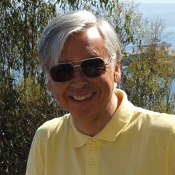
\includegraphics[width=0.9\textwidth]{img/salinas}
    \end{column}
    \begin{column}{0.3\textwidth}
            \begin{itemize}
                \item Dr. Luis Salinas
                \item \gray{Director}
            \end{itemize}
    \end{column}
%\end{columns}
%\hfill
%\vspace{0.2cm}
%\hfill
%\begin{columns}[T]
    \begin{column}{0.15\textwidth}
        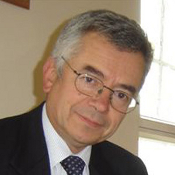
\includegraphics[width=0.9\textwidth]{img/canas}
    \end{column}
    \begin{column}{0.4\textwidth}
            \begin{itemize}
                \item M.Sc. Javier Cañas
                \item \gray{Sub Director}
            \end{itemize}
    \end{column}
\end{columns}
\hfill
\vspace{0.5cm}
\hfill
\begin{columns}
    \begin{column}{0.4\textwidth}
        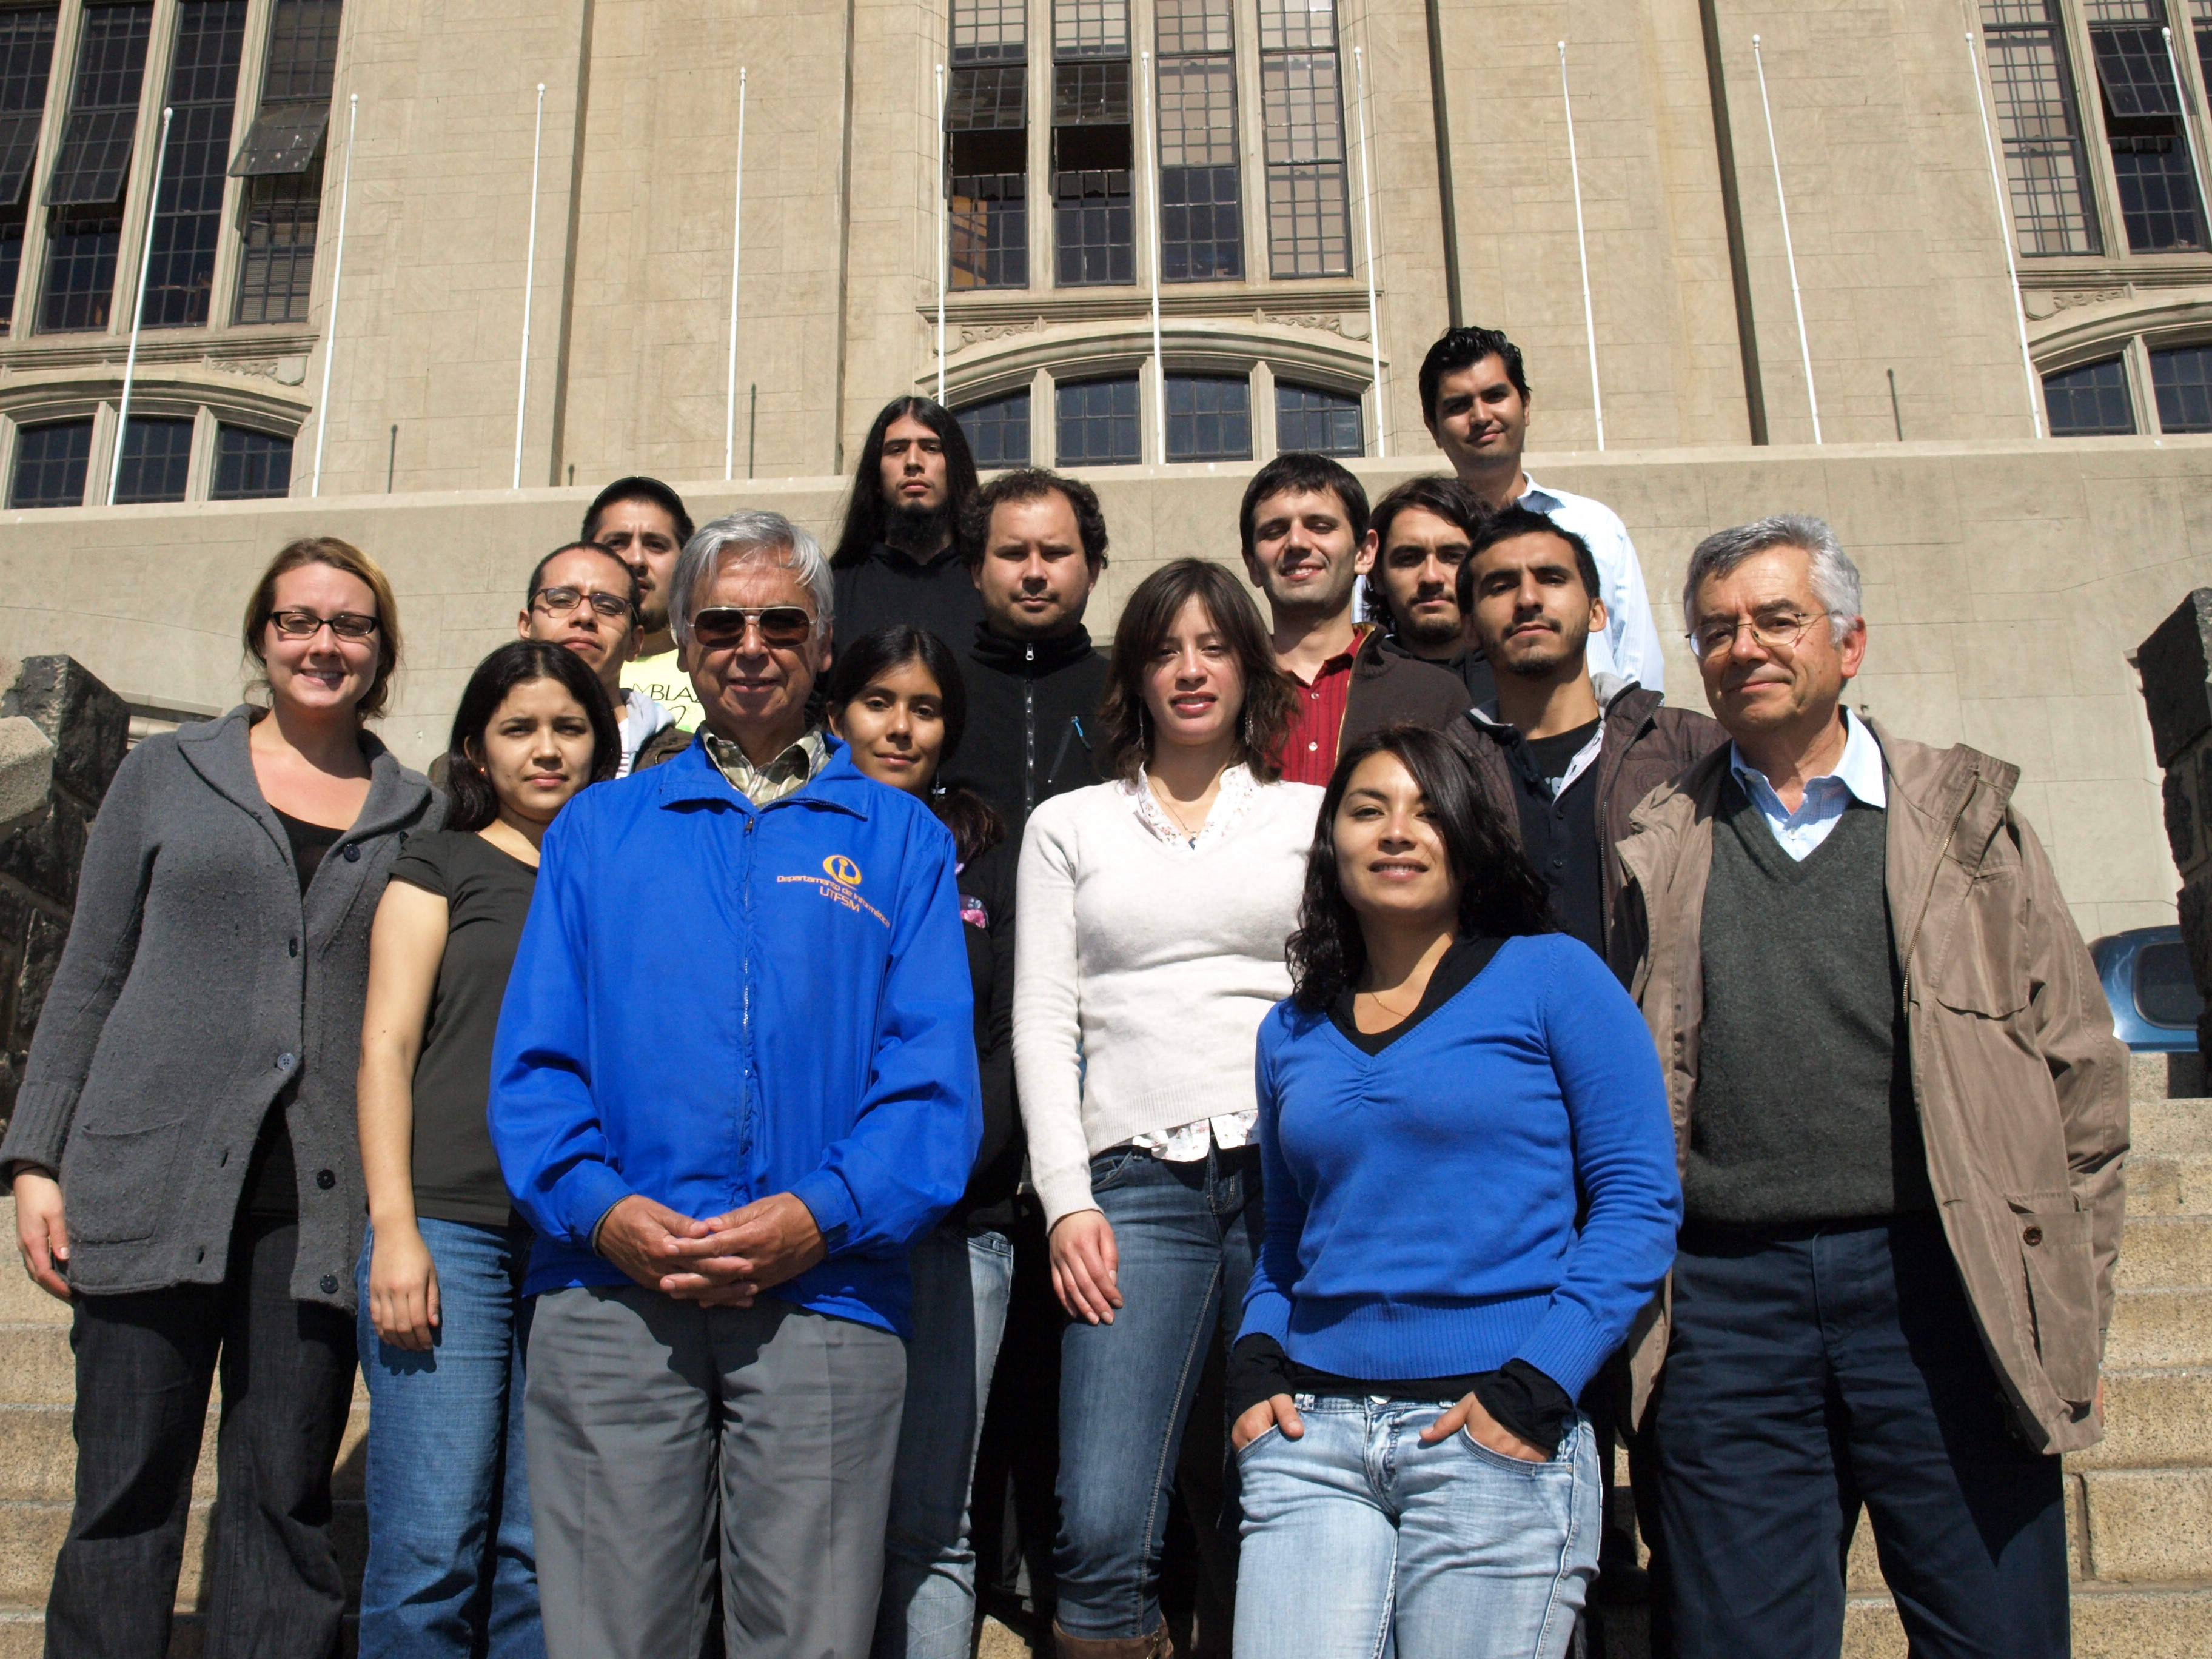
\includegraphics[width=0.9\textwidth]{img/equipo}
    \end{column}
    \begin{column}{0.6\textwidth}
        \begin{itemize}
            \item Investigadores de los programas
            \begin{itemize}
                \item Doctorado y Magister en Ciencias de la Ingeniería Informática.
            \end{itemize}
        \end{itemize}
    \end{column}
\end{columns}

}

\frame
{
\frametitle{\oran{Finanzas}}

Nuestro centro provee soluciones financieras a nivel nacional e internacional.

Proyectos:


\begin{columns}
\column{0.4\textwidth}
\begin{itemize}
\item Implementación de algoritmos para predicción de indicadores finacieros que manejan grandes volúmenes de datos y requieren respuestas en micro segundos. Empresa: Pan Alpha Trading.
\end{itemize}
\column{0.6\textwidth}
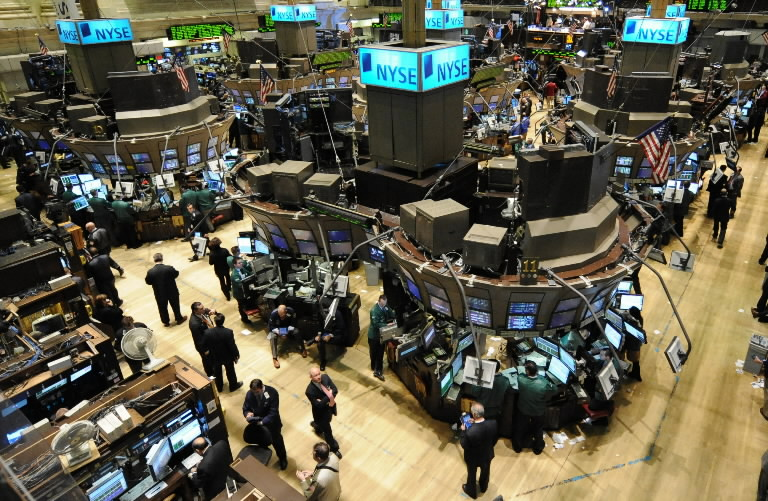
\includegraphics[width=0.7\textwidth]{img/wallstreet}
%\pgfuseimage{wallstreet}
\end{columns}

}

\frame
{
\frametitle{\oran{Finanzas}}

\begin{itemize}
\item Desarrollo de aplicación que permite la creación y edición de indices financieros, usando información actualizada diariamente, gran cantidad de activos y data histórica.
\end{itemize}
\begin{center}
 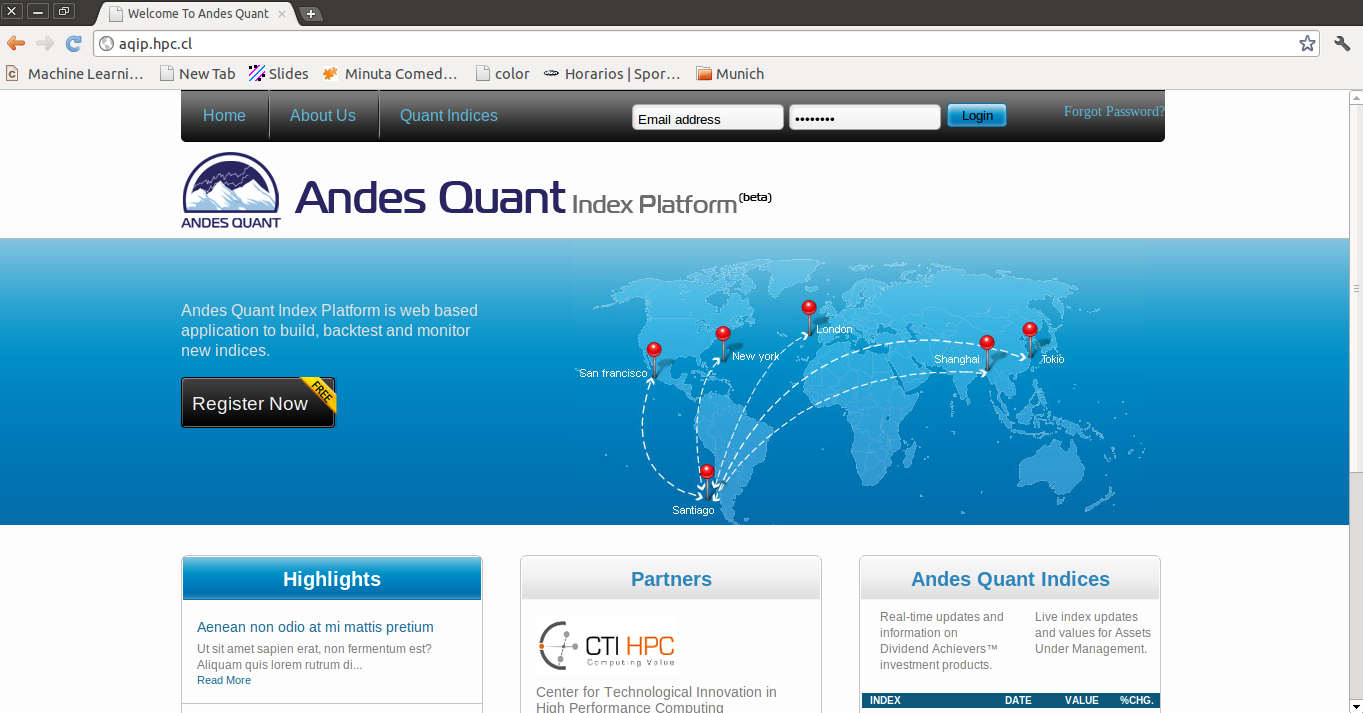
\includegraphics[width=0.7\textwidth]{img/ETF}
\end{center}





}


\frame
{
\frametitle{\oran{Finanzas Computacionales}}
 \begin{itemize}
	    \item Dise\~no e implementaci\'on de algoritmos de pron\'ostico de precios de alta frecuencia.
            \item Desarrollo de proyectos de software financiero:
	     \begin{itemize}
		  %\item Plataforma web para la mantenci\'on de \'indices financieros y Exchange Trade Fund (ETF).
		  \item Aplicaci\'on para el an\'alisis de \'indices financieros utilizando tecnolog\'ias 
			de alto desempe\~no orientadas a usuarios finales (Computaci\'on paralela heterog\'enea).
	      \end{itemize}
	      
\end{itemize}	     
\begin{center}
\pgfuseimage{volantin}
\end{center}
}


\frame{
\frametitle{\oran{Procesamiento de Imágenes}}
\framesubtitle{IHC-imágenes}
        \begin{columns}
        \column{0.5\textwidth}
	    \begin{itemize}
		
		\item IHC-imágenes: imágenes de tejidos tratados con la técnica
de inmunohistoquímica (IHC) \

\oran{\tiny{$\rightarrow$ Proyecto CCTVAl FB/14/RP/10}}

	        \begin{itemize}
               	\item Tejidos mamarios $\rightarrow$ sobrexpresión de la proteína HER2
	        	\begin{itemize} 
		        	\item \oran{Colaboración GISELA UFRO-UTFSM, Dr. Julio L\'{o}pez Fenner}
              		\end{itemize}
              	\item Tejidos cerebrales (ratones de laboratorio) $\rightarrow$ somas de neuronas
             \end{itemize}
	        
                \item Desarrollo de sistema web $\rightarrow$ desarrollo de filtros, usando computación paralela.

	    \end{itemize}

	\column{0.5\textwidth}

	   \pgfuseimage{ihc}
\\
            \pgfuseimage{neuronas}
\\
\tiny{Imágenes escaneadas en el TIGA Center, Heidelberg Universidad de Heidelberg}
        \end{columns}
}


\frame{
\frametitle{\oran{Procesamiento de Imágenes}}
\framesubtitle{Imágenes Satelitales}
\begin{itemize}
\item Colaboración: \textbf{O}ffice of \textbf{N}aval \textbf{R}esearch \textbf{G}lobal (ONRG).
\begin{itemize}
\item Desarrollo de escuelas de procesamiento de imágenes satelitales
$\rightarrow$ OSSIM software
\item Junto con Armada de Chile y organización privada $\rightarrow$ Maritime Domain Awareness (MDA).
\end{itemize}
\end{itemize}
\begin{center}
\pgfuseimage{ossim}
\end{center}
}

%

\frame
{
\frametitle{\oran{Bioinformática}}

\begin{columns}
\column{0.55\textwidth}
\begin{itemize}
\item FONDEF G09i1007,  \emph{Desarrollo y aplicaci\'{o}n de herramientas de gen\'{o}mica e ingenier\'{i}a gen\'{e}tica para potenciar el fitomejoramiento de vides de mesa}
\item Participantes:
	\begin{itemize}
	\item Coordinador: INIA
	\item Equipo bioinform\'{a}tico: 
		\begin{itemize}
		\item Dr. Alexander Zamyatnin (CTI-HPC, UTFSM)
		\item Dr. Francisco González (CTI-HPC, UVM)
		\end{itemize}
	\end{itemize}
\end{itemize}
\column{0.45\textwidth}
\begin{center}
\pgfuseimage{uva}
\end{center}
\end{columns}
}
% El objetivo del presente estudio es la identificación de nuevos oligopéptidos antimicrobianos con estudio funcional de las secuencias de proteínas de uva de Vitis vinifera.

%dedicada a mejorar la resistencia natural de los animales y las plantas contra hongos, patógenos y enfermedades.

\frame
{
\frametitle{\oran{Cuda Teaching Center}}
\begin{columns}
    \begin{column}{0.65\textwidth}
        \begin{itemize}
            \item Universidad nombrada oficialmente
            \begin{itemize}
                \item \gray{NVIDIA CUDA Teaching Center}
            \end{itemize}
            \item Primer CUDA Teaching Center en Chile.
            %Reconocimiento por la integración de técnicas de computación GPU en planes de estudio de las carreras del Departamento de Informática.
            \item Integración en planes de estudios.
            \begin{itemize}
                \item \gray{Primera Asignatura de HPC}
            \end{itemize}
            \item Donaciones de material académico y tarjetas NVIDIA.
        \end{itemize}
    \end{column}
    \begin{column}{0.35\textwidth}
        \begin{center}
            
\includegraphics[width=0.9\textwidth]{img/cuda_teaching}
        \end{center}
    \end{column}
\end{columns}
}

\frame
{
\frametitle{\oran{Capacitación y Difusión de HPC}}

%Apertura hacia nuevas áreas de investigación. Organización de eventos de carácter mundial, relacionados con HPC.

\begin{columns}
\column{0.6\textwidth}
\begin{itemize}
\item Eventos como:
\begin{itemize} 
\item  EPIKH (Exchange Programme to advance e-Infrastructure Know-How) $\rightarrow$ grid computing
\item SCAT (Scientific Computing-Advanced Training) y PASI (Panamerican Advanced Studies Institute) $\rightarrow$ computaci\'{o}n cient\'{i}fica y HPC
\end{itemize} 
garantizan 
la experticia generada, tanto a nivel organizativo como colaborativo. 
\item Instancia importante para capacitación de integrantes dentro del CTI-HPC. 
\end{itemize}
\column{0.4\textwidth}
\pgfuseimage{evento}
\end{columns}
}

\frame
{
\frametitle{\oran{Capacitación y Difusión de HPC}}

\begin{columns}
\column{0.6\textwidth}
\begin{itemize}
\item Cursos de programación para instituciones nacionales, Procesamiento de Imágenes Satelitales y desarrollo de aplicaciónes de Alto Desempeño sobre CUDA, permite la difusión de nuestras actividades.
\end{itemize}
\column{0.4\textwidth}
\pgfuseimage{curso}
\end{columns}

}



\frame
{
\frametitle{Infraestructura}
\framesubtitle{\oran{Data Center}}
El Data Center cuenta con 2 \emph{Clusters} y 4 Nodos GPU con las siguientes características:
\begin{table}[h]
\centering
\scalebox{0.7}{
  \begin{tabular}{|c|l|l|l|}
		\hline
					 & \textbf{Cluster 1} 		& \textbf{Cluster 2}		& \textbf{Nodos GPU} 		\\
		\hline
		\textbf{Nodos} 		 &12				&16				&4			\\
		\hline
		\textbf{CPU}		 &Dual Xeon 5110 1.60 GHz	&Dual Xeon X5560 2.8 GHz	&Dual Xeon E5520 2.27GHz\\
		\hline
		\textbf{RAM}		 &4GB				&16GB				&24GB			\\
		\hline
		\textbf{Storage}	 &12TB				&48TB				&250GB			\\
		\hline
		\textbf{GPU}		 &-				&-				&Tesla M2050		\\
		\hline
	\end{tabular}}
\caption{Características de los equipos}
\end{table}
%\begin{columns}
%\column{0.5 \textwidth}
%\begin{itemize}
%\item Actualmente se cuenta con dos \emph{Clusters} y 4 Nodos \emph{GPU}.
%\end{itemize}
%\column{0.5\textwidth}
%\pgfuseimage{utfsm}
%\end{columns}
}

\frame
{
\frametitle{Infraestructura}
\framesubtitle{\oran{Hacia donde vamos}}
\begin{itemize}
\item Se busca pasar de \emph{Tier-III} a \emph{Tier-II} en proyecto ATLAS.

\item En los próximos meses se instalará un nuevo Cluster parte del proyecto NLHPC, 
que cuenta con las siguientes características.

\end{itemize}
\begin{table}[h]
\centering
\scalebox{0.8}{
	\begin{tabular}{|c|l|}
		\hline
					 & \textbf{Cluster Proyecto NLHPC} 	\\
		\hline
		\textbf{Nodos} 		 &12					\\			
		\hline
		\textbf{CPU}		 &Dual Xeon X5675 3.06GHz		\\
		\hline
		\textbf{RAM}		 &32GB					\\
		\hline
		\textbf{Storage}	 &48TB					\\
		\hline
	\end{tabular}}
\caption{Características del Cluster Proyecto NLHPC}
\end{table}

}


\begin{frame}[t,plain]
\titlepage
\end{frame}
\end{document}
